% 1977 年广西卷第 2 题：圆外一点 P 的两条割线 P-D-B、P-C-A 与两条虚线弦 AD、BC（按源卷第 3 页布局）
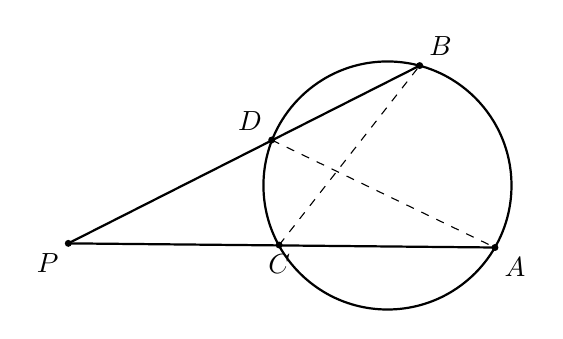
\begin{tikzpicture}[scale=1.05]
  % 圆
  \draw[thick] (0,0) circle (1.5);
  % 割线端点与圆上点（坐标手算：D、B、C、A 均在圆上，P 在圆外）
  \coordinate (P) at (-3.86,-0.70);
  \coordinate (D) at (-1.40,0.55);
  \coordinate (B) at (0.39,1.45);
  \coordinate (C) at (-1.31,-0.72);
  \coordinate (A) at (1.30,-0.75);
  % 两条割线（整段直画，保证共线）
  \draw[thick] (P) -- (B);
  \draw[thick] (P) -- (A);
  % 两条虚线弦
  \draw[dashed] (D) -- (A);
  \draw[dashed] (C) -- (B);
  % 顶点与标注
  \fill (P) circle (1.2pt) node[below left] {$P$};
  \fill (D) circle (1.2pt) node[above left] {$D$};
  \fill (B) circle (1.2pt) node[above right] {$B$};
  \fill (C) circle (1.2pt) node[below] {$C$};
  \fill (A) circle (1.2pt) node[below right] {$A$};
\end{tikzpicture}
